% pnuthesis_me 샘플 파일 (PNU 기계공학부 학위논문 서식)
%
% 출처 및 변형 이력:
%   1) 원출처: 서울대학교 전기·컴퓨터공학부 학위논문 양식
%      (https://ee.snu.ac.kr/community/notice/academic?bm=v&bbsidx=48811)
%   2) 이를 바탕으로 PNU 대학원 일반 양식(pnuthesis)으로 변형된 템플릿
%   3) 본 파일은 위 템플릿을 다시 **부산대학교 기계공학부** 최신 안내에 맞춰 수정·보완한 버전
%      (참고: 기계공학부 공지 – https://me.pusan.ac.kr/new/sub05/sub01_02.asp?seq=3289&db=gradnotice)
%
% 클래스: pnuthesis_me (report 기반)
% 옵션  : [doctor|master], [korean|english]
%   예) 박사/국문  : \documentclass[doctor,korean]{pnuthesis_me}
%       석사/국문  : \documentclass[master,korean]{pnuthesis_me}
%
% 빌드: pdflatex + bibtex (latexmk 권장)
%   latexmk -pdf
%   (nomenclature 필요 시: makeindex thesis.nlo -s nomencl.ist -o thesis.nls)
%

% 석사는 master, 박사는 doctor
% 영문은 english, 국문은 korean
\documentclass[doctor, korean]{pnuthesis_me}

% UsePackages
\usepackage{lineno}
\usepackage{tikz}
\usetikzlibrary{shapes, shapes.geometric, arrows.meta, positioning, calc}

\usepackage{graphicx}
\graphicspath{{figures/}}

% 논문 작성을 위한 사전 준비과정
% 논문제목 (국문, 영문), 저자, 제출일, 심사일, 졸업일의 정보를 넣습니다.

% 논문제목을 넣습니다.
% 필히 한글제목과 영문제목 모두 넣어야 합니다.
\title[korean]{Latex으로 논문을 써봅시다}
\title[english]{Let's write a paper with Latex.}

% 저자 정보를 넣습니다.
% 국문성명, 영문성명 모두 넣어야 하며, 특히 국문성명의 경우는 글자사이에 space가 있는 것과 없는 것
% 두 가지 모두를 넣어줘야 합니다.
\author[korean]{야 옹 이 (제 미 나 이)}
\author[english]{Ong-i Ya (Gemini)}
\author[nospace]{야옹이 (제미나이)}

% 지도교수님의 성함을 넣습니다.
\adviser[korean]{고 양 이}
\adviser[english]{Yang-ii Go}
\adviser[nospace]{고양이}

% 논문 제출일, 논문 심사일을 한글(영문 논문일 경우 영어)로 넣습니다.
\examinationdate[korean]{2025년 11월 14일}
\examinationdate[english]{14, November, 2025}

% 졸업일을 영문식, 한글식 두 가지 방법 모두 넣습니다.
\gradyear[korean]{2026년 2월}
\gradyear[english]{FEBRUARY 2026}

% 심사위원
% 국문 이름
\committeeChair[korean]{요 루 시 카}
\committeeMemberA[korean]{카 더 가 든}
\committeeMemberB[korean]{마 파 두 부}
% 박사면 아래 두 줄도 사용
\committeeMemberC[korean]{심 사 안 해}
\committeeMemberD[korean]{연 구 더 해}

% lstlisting용 옵션
\lstset{
    basicstyle=\ttfamily\small,
    numbers=left,
    numberstyle=\scriptsize,
    frame=single,
    columns=fullflexible,
    breaklines=true,
    keywordstyle=\color{blue!70!black},
    commentstyle=\color{gray!70!black},
    stringstyle=\color{green!40!black},
    inputencoding=utf8
}

% 한글 로렘 출처
% http://guny.kr/stuff/klorem/

\abstracts[korean]{
	본 문서는 \LaTeX 을 처음 사용하여 학위 논문을 작성하는 연구자와 학생들을 위한 종합 튜토리얼입니다.
    학위 논문 양식에 맞춰 문서의 기본 구조를 설정하는 방법부터 시작하여, 복잡한 수식 입력, 그리고 논문의 필수 요소인 그림과 표를 삽입하고 본문에서 참조하는 방법까지 단계별로 상세히 설명합니다. 
    또한, 참고문헌 관리와 부록 작성 등 학위 논문 완성에 필요한 추가적인 요소들도 다룹니다. 
    이 튜토리얼을 통해 사용자는 \LaTeX 의 강력한 조판 능력을 활용하여 전문적이고 체계적인 학술 문서를 효율적으로 작성할 수 있게 될 것입니다.

    뭘 해볼거냐면요  1. Latex 환경 구성하기, 2. 섹션 구성하기, 3. 그림, 표 넣고 본문에서 참조하기, 4. tikz로 순서도 그리기, 5. 레퍼런스 달기 입니다.
    그리고 초록은 영어로도 써야 합니다.
    이게 맨 뒤 페이지에 들어가요.
}
\abstracts[english]{
    This document is a comprehensive tutorial for researchers and students who are new to writing a thesis using \LaTeX. It provides a step-by-step guide tailored for a thesis format, starting from setting up the basic document structure to entering complex mathematical equations, and inserting and referencing figures and tables, which are essential components of a thesis. Furthermore, it covers additional elements necessary for completing a thesis, such as reference management and appendix creation. Through this tutorial, users will be able to efficiently produce professional and well-structured academic documents by leveraging the powerful typesetting capabilities of \LaTeX.

}
% 문서의 시작
%
% 위의 정보들을 빠짐없이 채워넣고 document를 시작하면
% 외표지, 내표지(외표지와 동일), 인준지가 자동으로 생성됩니다.

% \linenumbers

\begin{document}
\renewcommand{\baselinestretch}{1.5}    % 본문의 줄간격 조정, 고치거나 삭제하지 마십시오.
\selectfont                             %

\changepage{5mm}{}{}{}{}{}{}{}{-5mm}    %%페이지 여백 재설정. 절대 고치거나 삭제하지 마십시오.

% Nomenclature 입력
\nomenclature{$a$}{가속도}
\nomenclature{$E$}{에너지}
\nomenclature{$\rho$}{밀도}

\makelists
% 본문의 시작

\chapter{개요}
.tex 파일에는 학위논문 작성 시 지침이 있으니 읽어보세요

\section{\LaTeX}
\LaTeX 은 복잡한 수식, 표, 그림이 포함된 문서를 안정적으로 조판할 수 있는 도구입니다.
워드나 한글은 What you see is what you get (WYSIWYG)이라고 나한테 보이는게 최종 출력물로 나오는 편집기에요.
Latex은 내가 서식에다가 plain text로 글을 쓰고 컴파일을 하면 text를 서식에 맞춰서 출력물로 바꿔줘요.
이걸 왜 쓰냐? 라고 묻는다면
\begin{enumerate}
    \item 워드, 한글에서 글 위치에 따라 그림이나 표가 이상한 곳으로 움직이거나 사라지는거, 페이지 많아지면 프로그램 무거워지는거, 다크모드 제대로 안해주는거, 붙여넣기 귀찮은거 등등 불만이 많음
    \item 위랑 이어지는데, 그래서 내가 논문 쓸때 스트레스 받는 일이 적음
    \item sci급 저널은 tex 포맷을 주는 곳이 많아서 나는 글만 쓰고 컴파일 해버리면 저널 포맷에 맞춘 문서가 튀어나옴. 리젝 먹으면 서식만 바꿔서 제출할 수 있다
    \item 수식, 그림, 표, 참고문헌 넘버링이랑 정렬이 자동으로 됨
    \item 수식, 순서도 만들때 ai한테 쓰라고 해도 거의 잘 해줌
    \item 주석 처리가 가능해서 좀 애매한데 버리기 싫은 문장들 앞에 \%{} 붙이면 출력물에선 안보이지만 나중에 수정해서 넣을 수도 있음. vscode 기준 단축키는 ctrl + / 또는 command + /
    \item 메모장으로도 쓸 수 있지만 vscode 같은 편집기 쓰면 수식 미리보기, pdf 파일 실시간 미리보기, 자동완성, 플러그인 사용이 가능해서 편의성이 굉장히 좋아짐
    \item zotero랑 연동 가능
\end{enumerate}

\section{튜토리얼 구조}
뭐할거임?
\begin{enumerate}[label=\arabic*.]
    \item \LaTeX 환경 구성하기
    \item 섹션과 장 구조 설계하기
    \item 그림과 표 삽입 및 본문 참조하기
    \item \texttt{TikZ}로 순서도 작성하기
    \item 참고문헌 데이터 관리하기
\end{enumerate}

\chapter{\LaTeX 환경 구성하기}
\section{배포판 선택}
Windows 사용자는 \href{https://miktex.org/}{MiKTeX}, macOS 사용자는 \href{https://tug.org/mactex/}{MacTeX}, 리눅스 사용자는 \href{https://www.tug.org/texlive/}{TeX Live}를 설치하면 대부분의 패키지를 즉시 활용할 수 있습니다.
패키지 많아서 첫 설치는 굉장히 오래 걸림.

\section{편집기와 빌드 도구}

VS Code + Zotero 쓰세요.

VS Code에서 확장 설치하세요.
왼쪽에 보면 아래 그림처럼 생긴게 확장임.
\begin{figure}[htbp]
    \centering
    
\includegraphics{ext.png}
    \label{fig:ext}
\end{figure}

필수:

\textbf{LaTeX Workshop}

옵션:

\textbf{Zotero LaTeX} zotero랑 latex 연동. 인용한 문헌으로 왔다갔다 할 수 있음.

\textbf{Codex} openAI 코딩 에이전트이긴 한데 GPT보다 논문처럼 컨텍스트가 긴 작업을 잘 처리하는듯?

\textbf{indent-rainbow} 들여쓰기에 색깔을 넣어줘서 기분이 좋아져요

\section{프로젝트 구조}
문서, 그림, 참고문헌 파일을 역할별로 디렉터리에 분리해 두면 논문이 길어져도 유지 보수가 수월합니다.
논문 섹션마다 별도의 tex 파일을 둘수도 있다는데 굳이 필요할까 싶긴 함.
\begin{itemize}
    \item 본문: \texttt{논문파일.tex}
    \item 그림: \texttt{figures/}
    \item 참고문헌 데이터: \texttt{refs.bib}
\end{itemize}


\chapter{장과 섹션 설계하기}
\section{계층 구조 정의}\label{sec:structure}
학위 논문은 \verb|\chapter| 아래에 \verb|\section|, \verb|\subsection| (, \verb|\subsubsection|)이 있는 구조임.
\begin{lstlisting}[language=TeX]
\chapter{Background}
\label{chap:background}
This chapter introduces the research motivation and problem statement.

\section{Related Work}
\label{sec:related}
Summaries of prior studies appear here.
\end{lstlisting}


일반적인 논문은 \verb|\section|, \verb|\subsection|, \verb|\subsubsection| 구조.
\begin{lstlisting}[language=TeX]
\section{Background}
\label{sec:background}
Introduction blah blah

\section{Method}
\label{sec:method}
Summaries of prior studies appear here.

\subsection{Modeling}
\label{ss:method}

\subsection{Algorithm}
\label{ss:algo}

\end{lstlisting}

\verb|\\label|을 추가하면 Section~\ref{sec:structure}과 같이 장 번호를 자동으로 참조할 수 있으며, 섹션과 그림에도 동일한 방식이 적용됩니다.


\chapter{수식, 그림, 표 삽입하기}

\section{수식 입력}
\texttt{amsmath} 패키지가 기본으로 포함되어 있으므로, 정렬된 수식이나 다단 수식 환경을 그대로 사용할 수 있습니다.

\begin{equation}\label{eq:Rey}
    \frac{\partial}{\partial x} \left( \frac{h^3}{12 \mu} \frac{\partial p}{\partial x} \right) + 
    \frac{\partial}{\partial z} \left( \frac{h^3}{12 \mu} \frac{\partial p}{\partial z} \right) = 
    \frac{U}{2} \frac{\partial h}{\partial x} +
    \frac{V}{2} \frac{\partial h}{\partial z} +
    \frac{\partial h}{\partial t},
\end{equation}

본문에서는 식~\ref{eq:Rey}과 같이 참조하면 됩니다.

\verb|\ref| 대신 \verb|\eqref| 쓰면 식 번호에 괄호가 붙음.
The velocity profile~$\mathbf{u}$ can be obtained from the pressure distribution~$\mathbf{p}$ using Eq.~\eqref{eq:vel}:
\begin{equation}\label{eq:vel}
    \mathbf{u} = \left( 
        \int_0^z \dfrac{\xi}{\mu} \, d\xi 
        - \dfrac{ \displaystyle\int_0^h \dfrac{\xi}{\mu} \, d\xi }{ \displaystyle\int_0^h \dfrac{1}{\mu} \, d\xi } 
        \int_0^z \dfrac{1}{\mu} \, d\xi 
        \right) \nabla{\mathbf{p}}
        + \dfrac{ \displaystyle\int_0^z \dfrac{1}{\mu} \, d\xi }{ \displaystyle\int_0^h \dfrac{1}{\mu} \, d\xi } \cdot \mathbf{U}
\end{equation}

그리고 \verb|\begin{equation}| 부분에 커서를 올리면 식이 보임.







\section{그림 넣기}
\texttt{figure} 환경을 사용하고, \texttt{graphicx} 패키지의 \verb|\\includegraphics| 명령을 통해 외부 이미지를 불러옵니다.

\verb|\begin{figure}|로 \texttt{figure} 환경을 만드는데 \verb|\begin{figure}[htbp]|처럼 뒤에 위치 지정하는 값을 붙일수도 있음.
안붙이면 latex이 알아서 위치 잡아줌(안붙여도 상관 없음)

\begin{figure}[htbp]
    \centering
    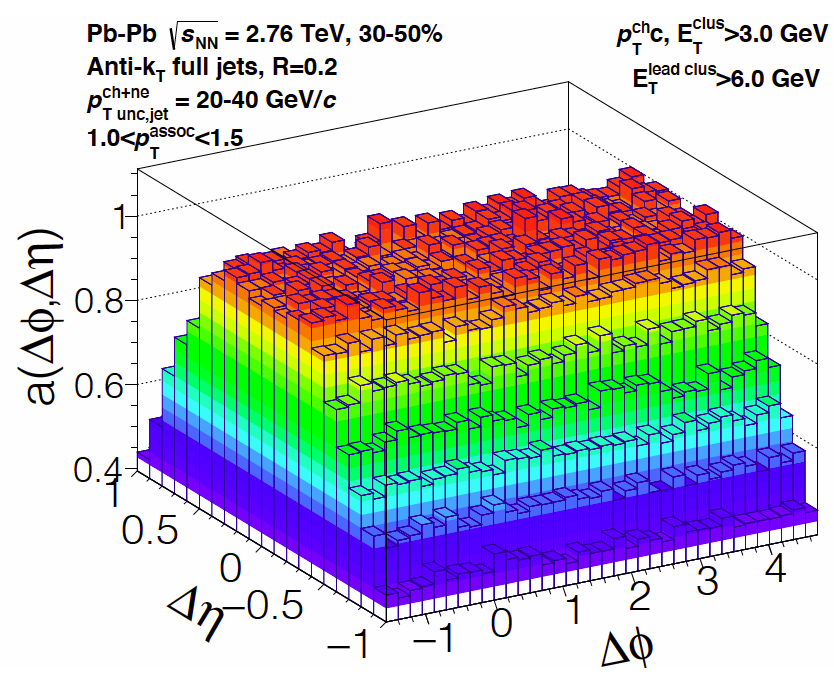
\includegraphics[width=0.5\textwidth]{samplefig1.png}
    \caption{예시 그림: 실제 작업에서는 \texttt{figures/} 폴더 내부 이미지를 삽입합니다.}
    \label{fig:example}
\end{figure}

그림~\ref{fig:example}처럼 캡션과 라벨을 함께 작성하면 본문에서 자동 번호를 이용해 참조할 수 있습니다.






\section{표 넣기}
표는 \texttt{table} 환경과 \texttt{tabular} 환경을 조합해 작성하며, 가독성을 위해 \texttt{booktabs} 패키지를 사용합니다.
\texttt{tabularx} 쓰면 표 밑에 노트 넣기 좋음.

\begin{table}[htbp]
    \centering
    \caption{성능 비교 예시 표}
    \label{tab:performance}
    \begin{tabular}{lccc}
        \toprule
        모델 & 정확도(\%) & 정밀도(\%) & 재현율(\%) \\
        \midrule
        제안 방법 & 94.8 & 93.1 & 95.6 \\
        비교 방법 A & 89.3 & 90.4 & 88.0 \\
        비교 방법 B & 91.7 & 88.9 & 92.5 \\
        \bottomrule
    \end{tabular}
\end{table}

표~\ref{tab:performance}는 자동으로 번호가 매겨지며, 긴 표에는 \texttt{longtable}이나 \texttt{tabularx}를 추가로 사용할 수 있습니다.





\chapter{\texttt{TikZ}로 순서도 그리기}
\texttt{TikZ}는 벡터 그래픽을 코드로 작성할 수 있게 해 주므로, 순서도와 블록 다이어그램 작성에 매우 유용합니다.

\begin{figure}[htbp]
    \centering
    \begin{tikzpicture}[
        node distance=12mm,
        every node/.style={draw, rounded corners, align=center, minimum width=32mm, minimum height=10mm},
        arrow/.style={-{Latex[length=3mm]}, line width=0.7pt}
        ]
        \node (start) {데이터 수집};
        \node (preprocess) [below=of start] {전처리};
        \node (train) [below=of preprocess] {모델 학습};
        \node (evaluate) [below=of train] {평가 및 검증};
        \node (deploy) [below=of evaluate] {배포};
        
        \draw[arrow] (start) -- (preprocess);
        \draw[arrow] (preprocess) -- (train);
        \draw[arrow] (train) -- (evaluate);
        \draw[arrow] (evaluate) -- (deploy);
    \end{tikzpicture}
    \caption{연구 절차 순서도 예시}
    \label{fig:workflow}
\end{figure}

복잡한 구조가 필요하다면 \texttt{backgrounds} 라이브러리와 \texttt{positioning} 옵션을 추가로 활용해 노드 배치를 세밀하게 제어할 수 있습니다.

\begin{figure}
\centering
\begin{tikzpicture}[
    node distance=1cm and 1.6cm,
    input/.style  ={rectangle,draw,fill=blue!10, rounded corners=3pt, minimum height=1cm, minimum width=3.2cm, align=center},
    layer/.style  ={rectangle,draw,rounded corners=3pt, minimum height=2cm, minimum width=1.0cm},
    head/.style   ={rectangle,draw,rounded corners=3pt, minimum height=0.6cm, minimum width=1.0cm}, % Head layer style
    branch/.style ={fill=orange!15},
    trunk/.style  ={fill=cyan!15},
    op/.style     ={circle,draw, fill=red!10, minimum size=8mm},
    output/.style ={rectangle,draw,fill=green!10, rounded corners=3pt, minimum height=8mm, minimum width=18mm, align=center},
    arrow/.style  ={-{Latex[length=2mm]}, thick},
    ]
    
    % --- Inputs (unchanged) ---
    \node[input] (branch_in) {피자};
    \node[font=\scriptsize, anchor = center] 
    at ($(branch_in.north)+(0mm,3mm)$) {파파존스};
    
    \node[input, below=3.2cm of branch_in] (trunk_in) {치킨};
    \node[font=\scriptsize, anchor = center] at ($(trunk_in.north)+(0mm,3mm)$) {파닭};
    
    % --- Branch Network (unchanged) ---
    \node[layer,branch, right=9mm of branch_in] (b1) {};
    \node[layer,branch, right=4mm of b1] (b2) {};

    % Multi head branch network
    \node[head,branch, right=8mm of b2, yshift=1.2cm] (b3_K) {};
    \node[head,branch, right=8mm of b2, yshift=0.4cm] (b3_k) {};
    \node[head,branch, right=8mm of b2, yshift=-0.4cm] (b3_C) {};
    \node[head,branch, right=8mm of b2, yshift=-1.2cm] (b3_c) {};
    \draw[dashed, gray, rounded corners]
        ([xshift=-3mm,yshift=2mm]b1.west |- b3_K.north) 
        rectangle
        ([xshift=3mm,yshift=-2mm]b3_c.south east);
    \node[font=\small, anchor=south west] 
        at ([xshift=-3mm,yshift=2mm]b1.west |- b3_K.north) {간장게장};

    % --- Trunk Network ---
    \node[layer, trunk, right=9mm of trunk_in] (t1) {};
    \node[layer, trunk, right=6mm of t1] (t2) {};
    \node[layer, trunk, right=6mm of t2] (t3) {};

    \draw[dashed, gray, rounded corners] ($(t1.north west)+(-3mm,2mm)$) rectangle ($(t3.south east)+(3mm,-2mm)$);
    \node[font=\small, anchor=south west] at ($(t1.north west)+(-3mm,3mm)$) {양념게장};
    
    \coordinate (branch_box) at ($(b3_K.north east)+(3mm,4mm)$);
    \coordinate (trunk_box) at ($(t3.south east)+(3mm,-2mm)$);
    \coordinate (center_line) at ($(branch_box)!0.5!(trunk_box)$);

    % --- Multiple Dot Products ---
    \node[op] (dot_k) at (center_line -| b3_K.east) [xshift=20mm, yshift=0.4cm] {$\times{}$};
    \node[op, above=0.4cm of dot_k] (dot_K) {$\times{}$};
    \node[op, below=0.4cm of dot_k] (dot_C) {$\times{}$};
    \node[op, below=0.4cm of dot_C] (dot_c) {$\times{}$};
    
    % --- Outputs (MODIFIED positioning slightly) ---
    \node[output, right=8mm of dot_K] (outK) {삼겹살};
    \node[output, right=8mm of dot_k] (outk) {목살};
    \node[output, right=8mm of dot_C] (outC) {차돌박이};
    \node[output, right=8mm of dot_c] (outc) {스팸};
    \node[font=\small, anchor=north] at ($(outK.north)+(0mm,6mm)$) {김참맛-김치가 참 맛있는 집};
    
    % --- Connections (MODIFIED) ---
    \draw[arrow] (branch_in) -- (b1);
    \draw[arrow] (b1) -- (b2);
    % Branch heads to corresponding dots
    \coordinate (b_hub) at ($(b2.east)+(4mm,0)$);

    \draw[arrow] (b2.east) -- (b_hub);
    \draw[arrow] (b_hub) |- (b3_K.west);
    \draw[arrow] (b_hub) |- (b3_k.west);
    \draw[arrow] (b_hub) |- (b3_C.west);
    \draw[arrow] (b_hub) |- (b3_c.west);

    
    \draw[arrow] (b3_K.east) -- (dot_K.west);
    \draw[arrow] (b3_k.east) -- (dot_k.west);
    \draw[arrow] (b3_C.east) -- (dot_C.west);
    \draw[arrow] (b3_c.east) -- (dot_c.west);
    
    % Trunk to all dots
    \draw[arrow] (trunk_in) -- (t1);
    \draw[arrow] (t1) -- (t2);
    \draw[arrow] (t2) -- (t3);

    \draw[arrow] (t3.east) -- (dot_K.west);
    \draw[arrow] (t3.east) -- (dot_k.west);
    \draw[arrow] (t3.east) -- (dot_C.west);
    \draw[arrow] (t3.east) -- (dot_c.west);

    % Dots to outputs
    \draw[arrow] (dot_K) -- (outK);
    \draw[arrow] (dot_k) -- (outk);
    \draw[arrow] (dot_C) -- (outC);
    \draw[arrow] (dot_c) -- (outc);

\end{tikzpicture}
\caption{피자는 파파존스, 김치찜은 김참맛+고기 추가}
\label{fig:배고프다}
\end{figure}

\chapter{참고문헌 관리하기}
\section{BibTeX 활용}
참고문헌 데이터는 \texttt{.bib} 파일에 저장하고, 본문에서는 \verb|\cite{}| 명령을 통해 호출합니다~\cite{childsFiniteLengthSolutionsRotordynamic1983}..

\verb|\cite{}|까지 쓰면 bib에 있는 논문의 citation key가 나와요.
나는 Zotero: Add citation 기능으로 참고문헌 불러오기가 잘 안돼서 zotero에서 bib을 복사해서 refs.bib에 붙여넣음.



%
% 참고문헌
%
\bibliographystyle{unsrt} 
\bibliography{refs}

\appendix
\chapter{나머지는 생각나면 추가할 것}
입니다

\pagebreak


\acknowledgement 

왕감사합니다.

아리가토고자이마스.

\end{document}
